\documentclass[12pt]{ctexart}
\usepackage[sectionbib]{natbib}

\CTEXsetup[format={\bfseries\raggedright}]{section}


\renewcommand{\baselinestretch}{1.2}
\textwidth=33.9pc
\textheight=46.5pc
%\oddsidemargin=1pc
%\evensidemargin=1pc
\headsep=15pt
%\headheight=.2cm
\topmargin=.6cm
\parindent=1.7pc
\parskip=0pt
\usepackage{type1cm}
\usepackage{times}

\usepackage{caption}
\usepackage{graphicx, subfig}
\usepackage{amsmath}
\usepackage{amssymb}
\usepackage{amsfonts}
\usepackage{multirow}
\usepackage{amsthm}
\usepackage{setspace}
\usepackage{etoolbox}

\setcounter{page}{1}
\newtheorem{theorem}{定理}
\newtheorem{lemma}{引理}
\newtheorem{corollary}{推论}
\newtheorem{proposition}{命题}

\newtheorem{definition}{定义}
%\newtheorem{proof}{Proof}
\newtheorem{example}{Example}
\newtheorem{remark}{Remark}



%% recommended packages
\usepackage{thumbpdf,lmodern}
%% another package (only for this demo article)
\usepackage{framed}
\usepackage{fancyheadings}
\usepackage{rotating}
\usepackage[]{hyperref}  %<----modified by Ivan
\usepackage{amsmath,mathtools}
\usepackage{etoolbox}
\usepackage{pdfsync}



%% new custom commands
\newcommand{\class}[1]{`\code{#1}'}
\newcommand{\fct}[1]{\code{#1()}}
\newcommand{\ba}{\mbox{\bf a}}
\newcommand{\bb}{\mbox{\bf b}}
\newcommand{\bc}{\mbox{\bf c}}
\newcommand{\be}{\mbox{\bf e}}
\newcommand{\bff}{\mbox{\bf f}}
\newcommand{\bg}{\mbox{\bf g}}
\newcommand{\bt}{\mbox{\bf t}}
\newcommand{\bh}{\mbox{\bf h}}
\newcommand{\br}{\mbox{\bf r}}
\newcommand{\bu}{\mbox{\bf u}}
\newcommand{\bv}{\mbox{\bf v}}
\newcommand{\bw}{\mbox{\bf w}}
\newcommand{\bx}{\mbox{\bf x}}
\newcommand{\by}{\mbox{\bf y}}
\newcommand{\bz}{\mbox{\bf z}}
\newcommand{\bA}{\mbox{\bf A}}
\newcommand{\bB}{\mbox{\bf B}}
\newcommand{\bC}{\mbox{\bf C}}
\newcommand{\bT}{\mbox{\bf T}}
\newcommand{\bD}{\mbox{\bf D}}
\newcommand{\bd}{\mbox{\bf d}}
\newcommand{\bE}{\mbox{\bf E}}
\newcommand{\bF}{\mbox{\bf F}}
\newcommand{\bG}{\mbox{\bf G}}
\newcommand{\bH}{\mbox{\bf H}}
\newcommand{\bI}{\mbox{\bf I}}
\newcommand{\bK}{\mbox{\bf K}}
\newcommand{\bJ}{\mbox{\bf J}}
\newcommand{\bL}{\mbox{\bf L}}
\newcommand{\bP}{\mbox{\bf P}}
\newcommand{\bQ}{\mbox{\bf Q}}
\newcommand{\bM}{\mbox{\bf M}}
\newcommand{\bR}{\mbox{\bf R}}
\newcommand{\Rcal}{\mbox{$\mathcal{R}$}}
\newcommand{\Gcal}{\mbox{$\mathcal{G}$}}
\newcommand{\bS}{S}
\newcommand{\bU}{\mbox{\bf U}}
\newcommand{\bV}{\mbox{\bf V}}
\newcommand{\bW}{\mbox{\bf W}}
\newcommand{\bX}{\mbox{\bf X}}
\newcommand{\bXM}{\mbox{\bf X}_{\widehat{\mathcal{M}}}}
\newcommand{\bY}{\mbox{\bf Y}}
\newcommand{\bZ}{\mbox{\bf Z}}
\newcommand{\bone}{\mbox{\bf 1}}
\newcommand{\bzero}{\mbox{\bf 0}}
\newcommand{\bveps}{\mbox{\boldmath $\varepsilon$}}
\newcommand{\beps}{\mbox{\boldmath $\epsilon$}}
\newcommand{\balpha}{\mbox{\boldmath $\alpha$}}
\newcommand{\blambda}{\mbox{\boldmath $\lambda$}}
\newcommand{\bTheta}{\mbox{\boldmath $\Theta$}}
\newcommand{\bbeta}{\mbox{\boldmath $\beta$}}
\newcommand{\btheta}{\mbox{\boldmath $\theta$}}
\newcommand{\bgamma}{\mbox{\boldmath $\gamma$}}
\newcommand{\bGamma}{\mbox{\boldmath $\Gamma$}}
\newcommand{\bPi}{\mbox{\boldmath $\Pi$}}
\newcommand{\bPsi}{\mbox{\boldmath $\Psi$}}
\newcommand{\bet}{\mbox{\boldmath $\eta$}}
\newcommand{\bxi}{\mbox{\boldmath $\xi$}}
%\newcommand{\bleta}{\mbox{\boldmath $\eta$}}
\newcommand{\bvarphi}{\mbox{\boldmath $\varphi$}}
\newcommand{\bmu}{\mbox{\boldmath $\mu$}}
\newcommand{\bzeta}{\mbox{\boldmath $\zeta$}}
\newcommand{\bomega}{\mbox{\boldmath $\omega$}}
\newcommand{\bOmega}{\mbox{\boldmath $\Omega$}}
\newcommand{\bvphi}{\mbox{\boldmath $\varphi$}}
\newcommand{\bvarepsilon}{\mbox{\boldmath $\varepsilon$}}
\newcommand{\bSigma}{\mbox{\boldmath $\Sigma$}}
\newcommand{\bDelta}{\mbox{\boldmath $\Delta$}}
\newcommand{\hbv}{\widehat{\bv}}
\newcommand{\hB}{\widehat \bB}
\newcommand{\hE}{\widehat \bE}
\newcommand{\hvar}{\widehat \var}
\newcommand{\hcov}{\widehat \cov}
\newcommand{\hbveps}{\widehat\bveps}
\newcommand{\hbbeta}{\widehat\bbeta}
\newcommand{\hgamma}{\widehat\gamma}
\newcommand{\tgamma}{\widetilde\gamma}
\newcommand{\tbbeta}{\widetilde\bbeta}
\newcommand{\tbeta}{\widetilde\beta}
\newcommand{\hbgamma}{\widehat\bgamma}
\newcommand{\tbgamma}{\widetilde\bgamma}
\newcommand{\hbeta}{\widehat\beta}
\newcommand{\hSig}{\widehat\Sig}
\newcommand{\hbmu}{\widehat\bmu}
\newcommand{\hmu}{\widehat\mu}
\newcommand{\hxi}{\widehat\bxi}
\newcommand{\tSig}{\widetilde\Sig}
\newcommand{\heq}{\ \widehat=\ }
\newcommand{\mathcalR}{\mathcal{R}}
\newcommand{\mathcalG}{\mathcal{G}}
\newcommand{\Mfrak}{\mathfrak{M}}
\newcommand{\bMfrak}{\overline{\mathfrak{M}}}
\newcommand{\hbP}{\widehat{\bP}}
\newcommand{\hbV}{\widehat{\bV}}
\newcommand{\hRcal}{\widehat{\Rcal}}
\newcommand{\hGcal}{\widehat{\Gcal}}
\newcommand{\hbT}{\widehat{\bT}}

\newcommand{\std}{\mathrm{std}}
\newcommand{\var}{\mathrm{var}}
\newcommand{\cov}{\mathrm{cov}}
\newcommand{\corr}{\mathrm{corr}}
\newcommand{\Sig}{\mathbf{\Sigma}}
\newcommand{\veps}{\varepsilon}
\newcommand{\tr}{\mathrm{tr}}
\newcommand{\diag}{\mathrm{diag}}
\newcommand{\vecc}{\mathrm{vec}}
\newcommand{\vech}{\mathrm{vech}}
\newcommand{\rank}{\mathrm{rank}}
\newcommand{\sgn}{\mathrm{sgn}}
\newcommand{\supp}{\mathrm{supp}}
\newcommand{\lammin}{\lambda_{\text{min}}}
\newcommand{\lammax}{\lambda_{\text{max}}}
\newcommand{\D}{\scriptstyle}
\newcommand{\GIC}{\mbox{GIC}}

\def\t{^{\mathrm{\scriptscriptstyle T}}}
\def\toD{\overset{\mathscr{D}}{\longrightarrow}}
\def\toP{\overset{\mathrm{P}}{\longrightarrow}}
\def\toas{\overset{\mathrm{a.s.}}{\longrightarrow}}
\newcommand{\etal}{{\it et al.}}
\def\deq{\overset{\mathrm{(d)}}{=\hspace{-0.02 in}=}}

\def\e{\varepsilon}
\def\beq{\begin{equation}}
\def\eeq{\end{equation}}

\renewcommand{\theequation}{\arabic{section}.\arabic{equation}}

\renewcommand{\d}{\textrm {d}}


\title{美国枪击数据研究}

\author{马逸铭  SA20017054}
\date{}


\begin{document}

\maketitle

\begin{abstract}
 本文综合运用各种统计方法分析了美国从2014年1月1日到2018年3月31日的所有的枪击案数据,分析的角度包括从枪击案发生的频率、时间维度以及空间维度,并且综合运用了参数方法核非参数方法。在从发生频率分析枪击案数据时,运用了参数法拟合也运用了各种核密度方法拟合;在从时间维度分析时,运用了时间序列方法、核回归方法、样条回归方法、GAM模型多角度分析对比。从空间维度分析时,运用多维核密度估计法,得到了高发地的分布。这位进一步的现实意义下的分析提供了统计学上的支持。

\noindent {\it 关键词:} 核密度估计;样条光滑;非参数方法

\end{abstract}





\section{数据和问题描述}
此部分介绍数据和所研究的问题。
\subsection{数据来源特点}
本文数据来自于https://github.com/jamesqo/gun-violence-data,源数据由枪支暴力档案馆GVA)提供,该公司是一家不以营利为目的的公司,成立于 2013 年,为公众提供免费在线在线访问有关美国枪支相关暴力的准确信息。GVA 将收集和检查有关美国枪支相关暴力的准确性、全面信息,然后在网上发布和传播。
该数据集包括了了2013年1月到2018年3月的枪击案数据,但是2013年数据缺失太多,所以在本文分析中删去,该数据集案件的编号,发生日期,死伤人数。大部分部分包含枪击发生的经纬度,在分析空间规律时删去缺失经纬度数据的样本。除此外还包括案件具体的网页的链接。

\subsection{问题描述}
由于历史原因,美国形成了根深蒂固的枪支文化,美国枪击案爆发频率越来越高,枪支暴力事件远超世界上其他发达国家。美国人拥有约2.65亿支枪,平均每位成年人都有超过1支枪,所以美国的枪击事件频发,在数据集记录的从2013年1月到2018年3月发生了24万起枪击案件。在以往的分析中往往缺乏统计支持,所以本文想主要通过非参数方法分析数据并为进一步分析提供支持。


\section{模型与数据分析}

\subsection{枪击案发生频率}
由数据集可知美国枪击案发生的频率是是很高的,每天都会有枪击案报告登记在册,首先按日期统计后,得到每天发生的案件数。发现每天登记数量大多分布在100到200,所以我想进一步分析每天发生的枪击案的数量是呈一种什么样的分布。首先进行密度估计,这里由于不知道具体的分布,所以采用Histogram法,在带宽选取时,这里在$AIMSE$准则下,并取$h_{o p t}=c n^{-1 / 3}$,其中$ c $取正态假设下的$c \approx 3.5 \sigma$,得到了Histogram法的密度估计(见图一)。

\begin{figure}[!htb]
	\centering
	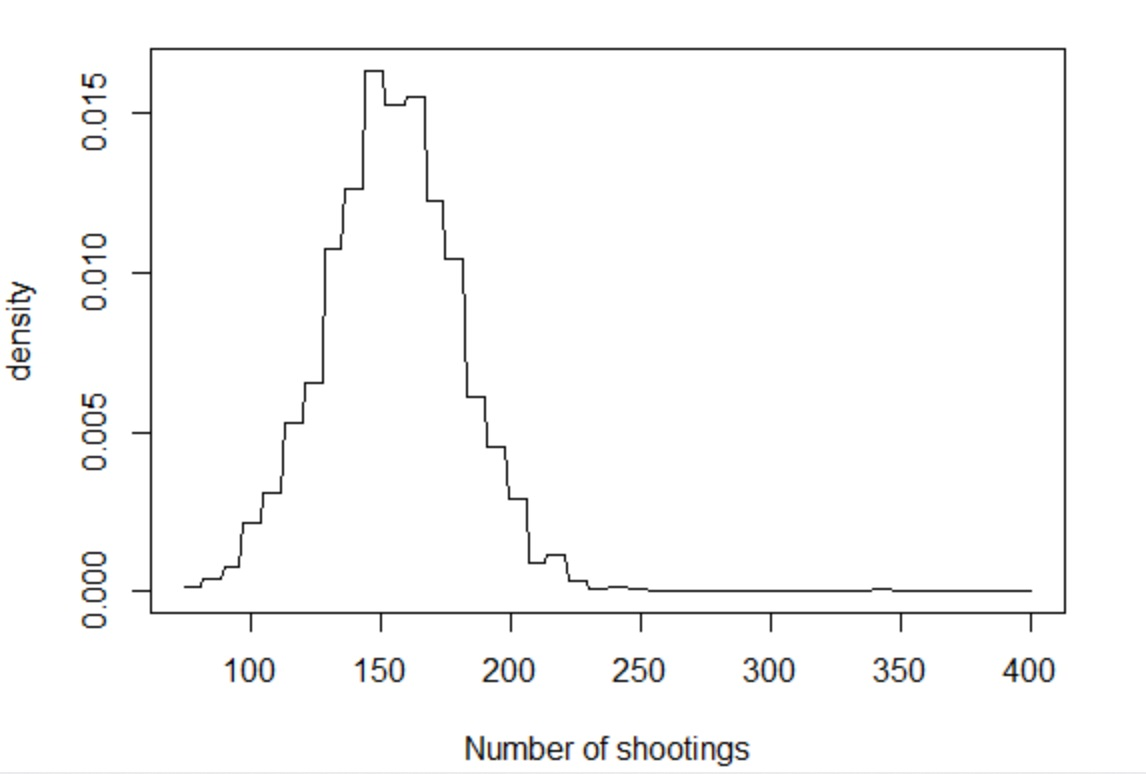
\includegraphics[width=.7\textwidth]{hist.jpg} %1.png是图片文件的相对路径
	\caption{Histogram估计的密度} %caption是图片的标题
\end{figure}

这种方法估计的密度不够光滑,所以观察到图象有一些像正态分布,所以进行正态性的检验,先画出Q-Q图(图二),
\begin{figure}[!htb]
	\centering
	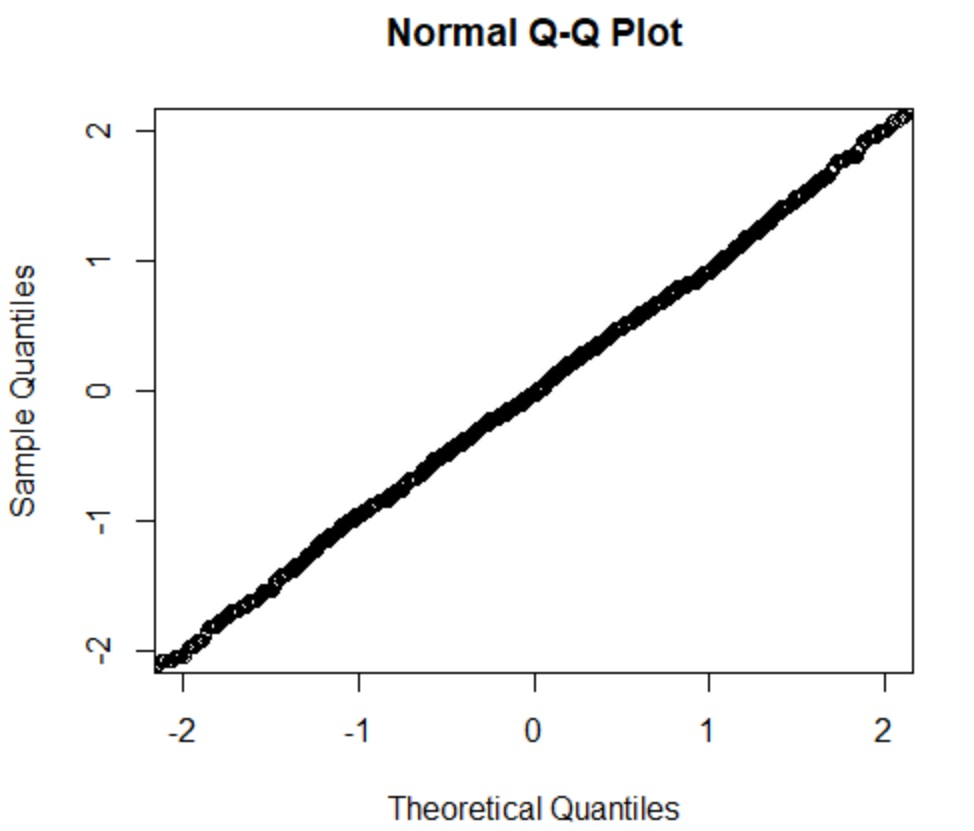
\includegraphics[width=.5\textwidth]{qqplot.jpg} %1.png是图片文件的相对路径
	\caption{Q-Q plot} %caption是图片的标题
\end{figure}
再进行shapiro test,得到结果$ W = 0.98918p,-value = 2.575 \times 10^{-9} $,W值十分接近1,且P值十分小,故考虑每日枪击案发生数量是呈正态分布,易得到其极大似然估计就是$ \mu = 154.6, \sigma = 25.8 $的正态分布,见(图三)。
\begin{figure}[!htb]
	\centering
	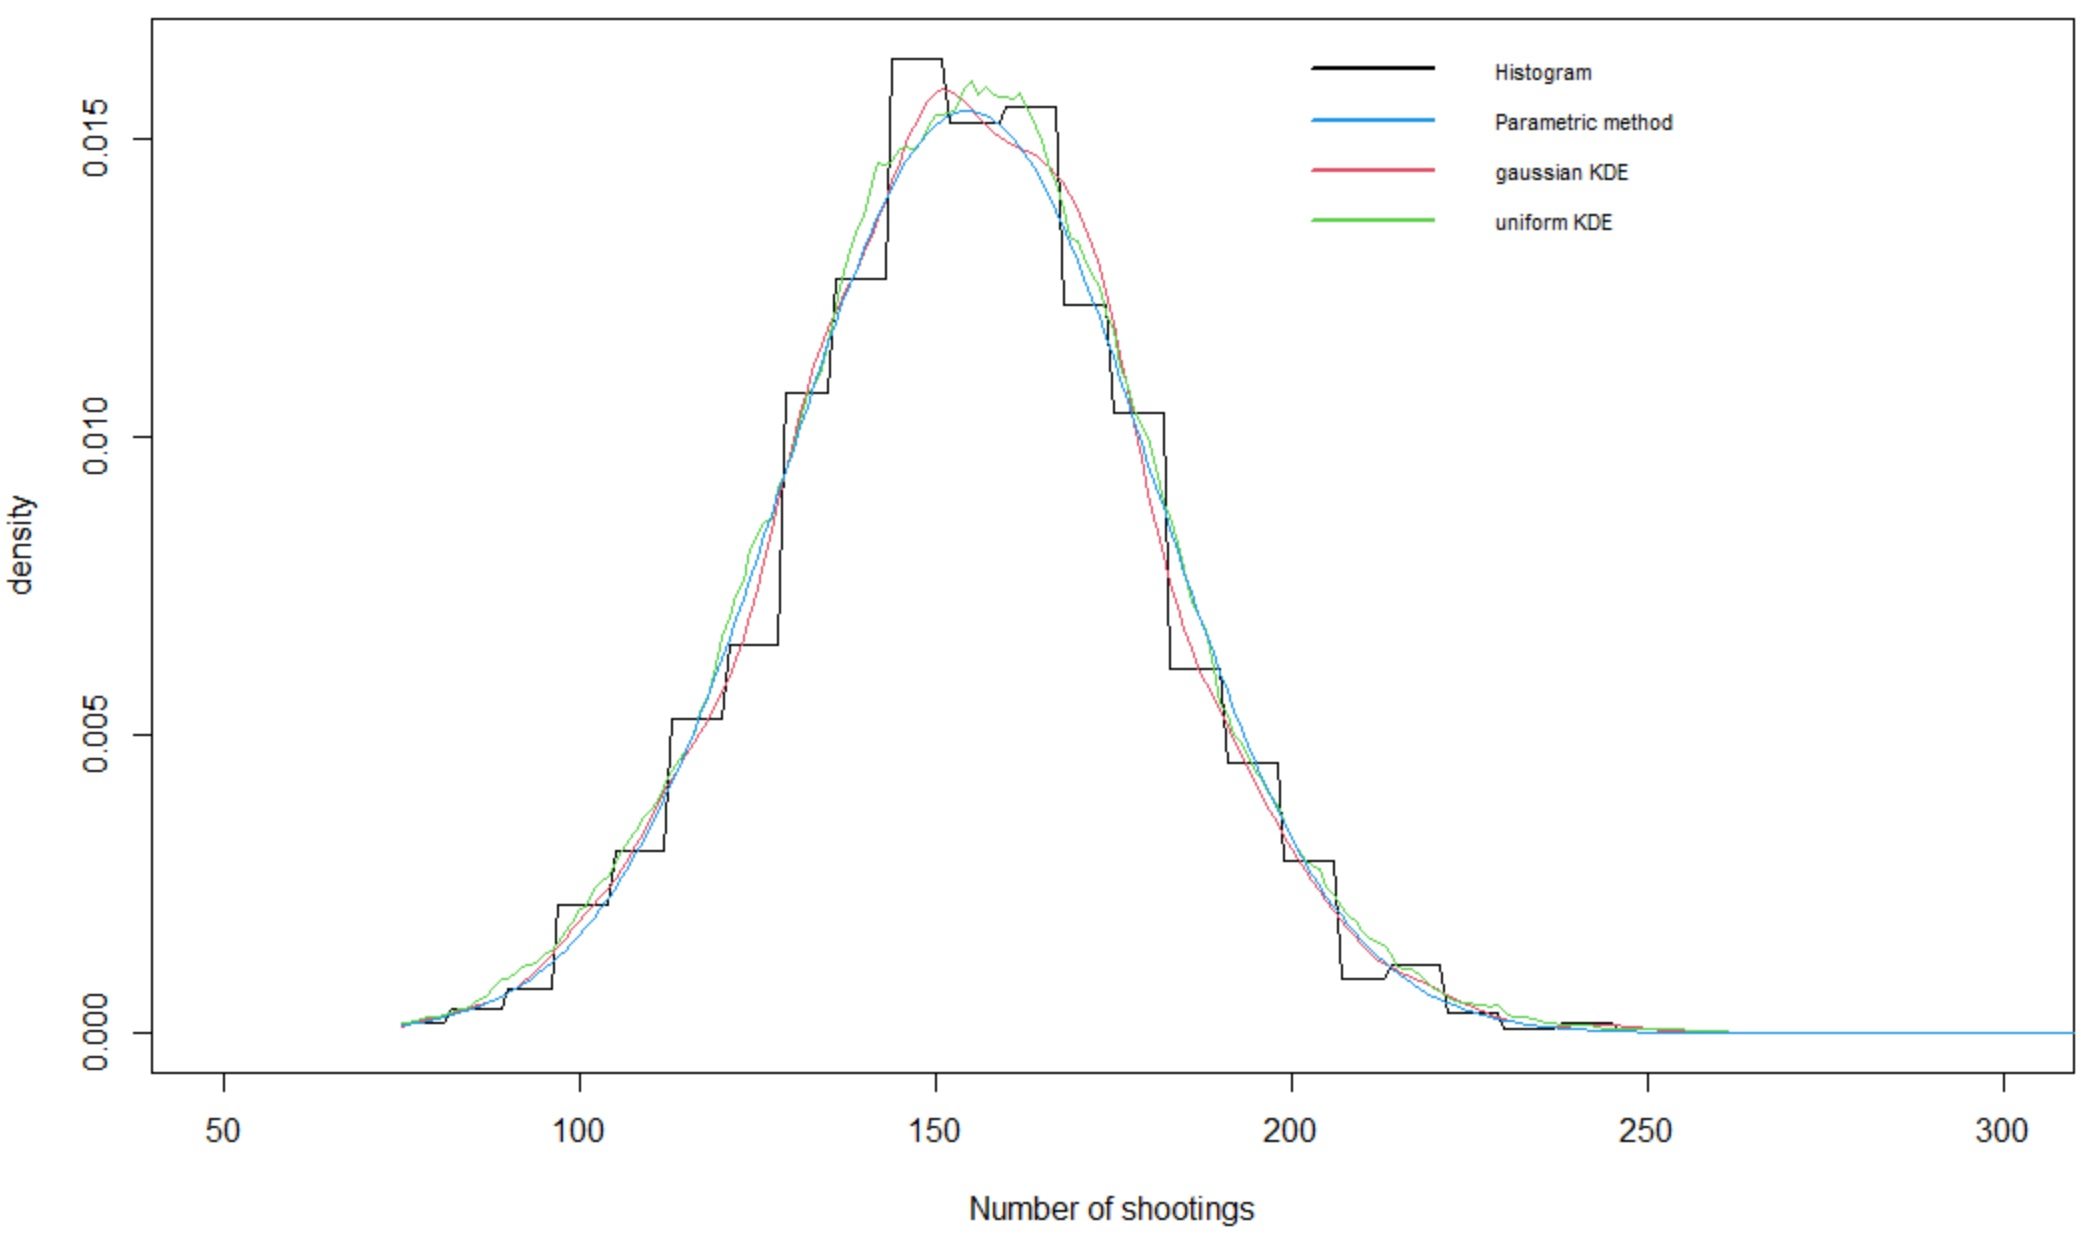
\includegraphics[width=0.7\textwidth]{kde.jpg} %1.png是图片文件的相对路径
	\caption{kde and parametric} %caption是图片的标题
\end{figure}

接下来考虑非参数方法的核密度估计,与参数法进行比较比较,这里考虑常见的简单核密度估计,即核函数是均匀分布与核函数是正态分布的情况。这里带宽选择均采取LSCV准则,即最小二乘交叉验证。并将图线画在图三中,发现在模型高度符合已知分布下,非参数法优势不明显,拟合结果区别不大。

\subsection{枪击案件的时间规律}

下面考虑枪击案数量随时间变化的规律,为了数据处理时的方便,将日期一一对应到非负整数。画出散点图,可以看出枪击案件数量的分布是波动很大,不光滑,这对研究其性质特点造成了困难,所以需要光滑。由于这是时间序列的数据,所以可以考虑移动平均法来光滑数据,因为数据波动频繁,单次移动平均效果可能不很好,可以考虑采取多次移动平均。并且和滑动中值法进行比较。移动平均法就是指将每个点前后若干个点进行平均作为该点光滑后取值,滑动中值法则是取前后若干点的中值作为光滑后该点取值。并且从图中可以看到枪击案件数量是增加趋势的,画出拟合直线图斜率为正。见图四。

\begin{figure}[!htb]
	\centering
	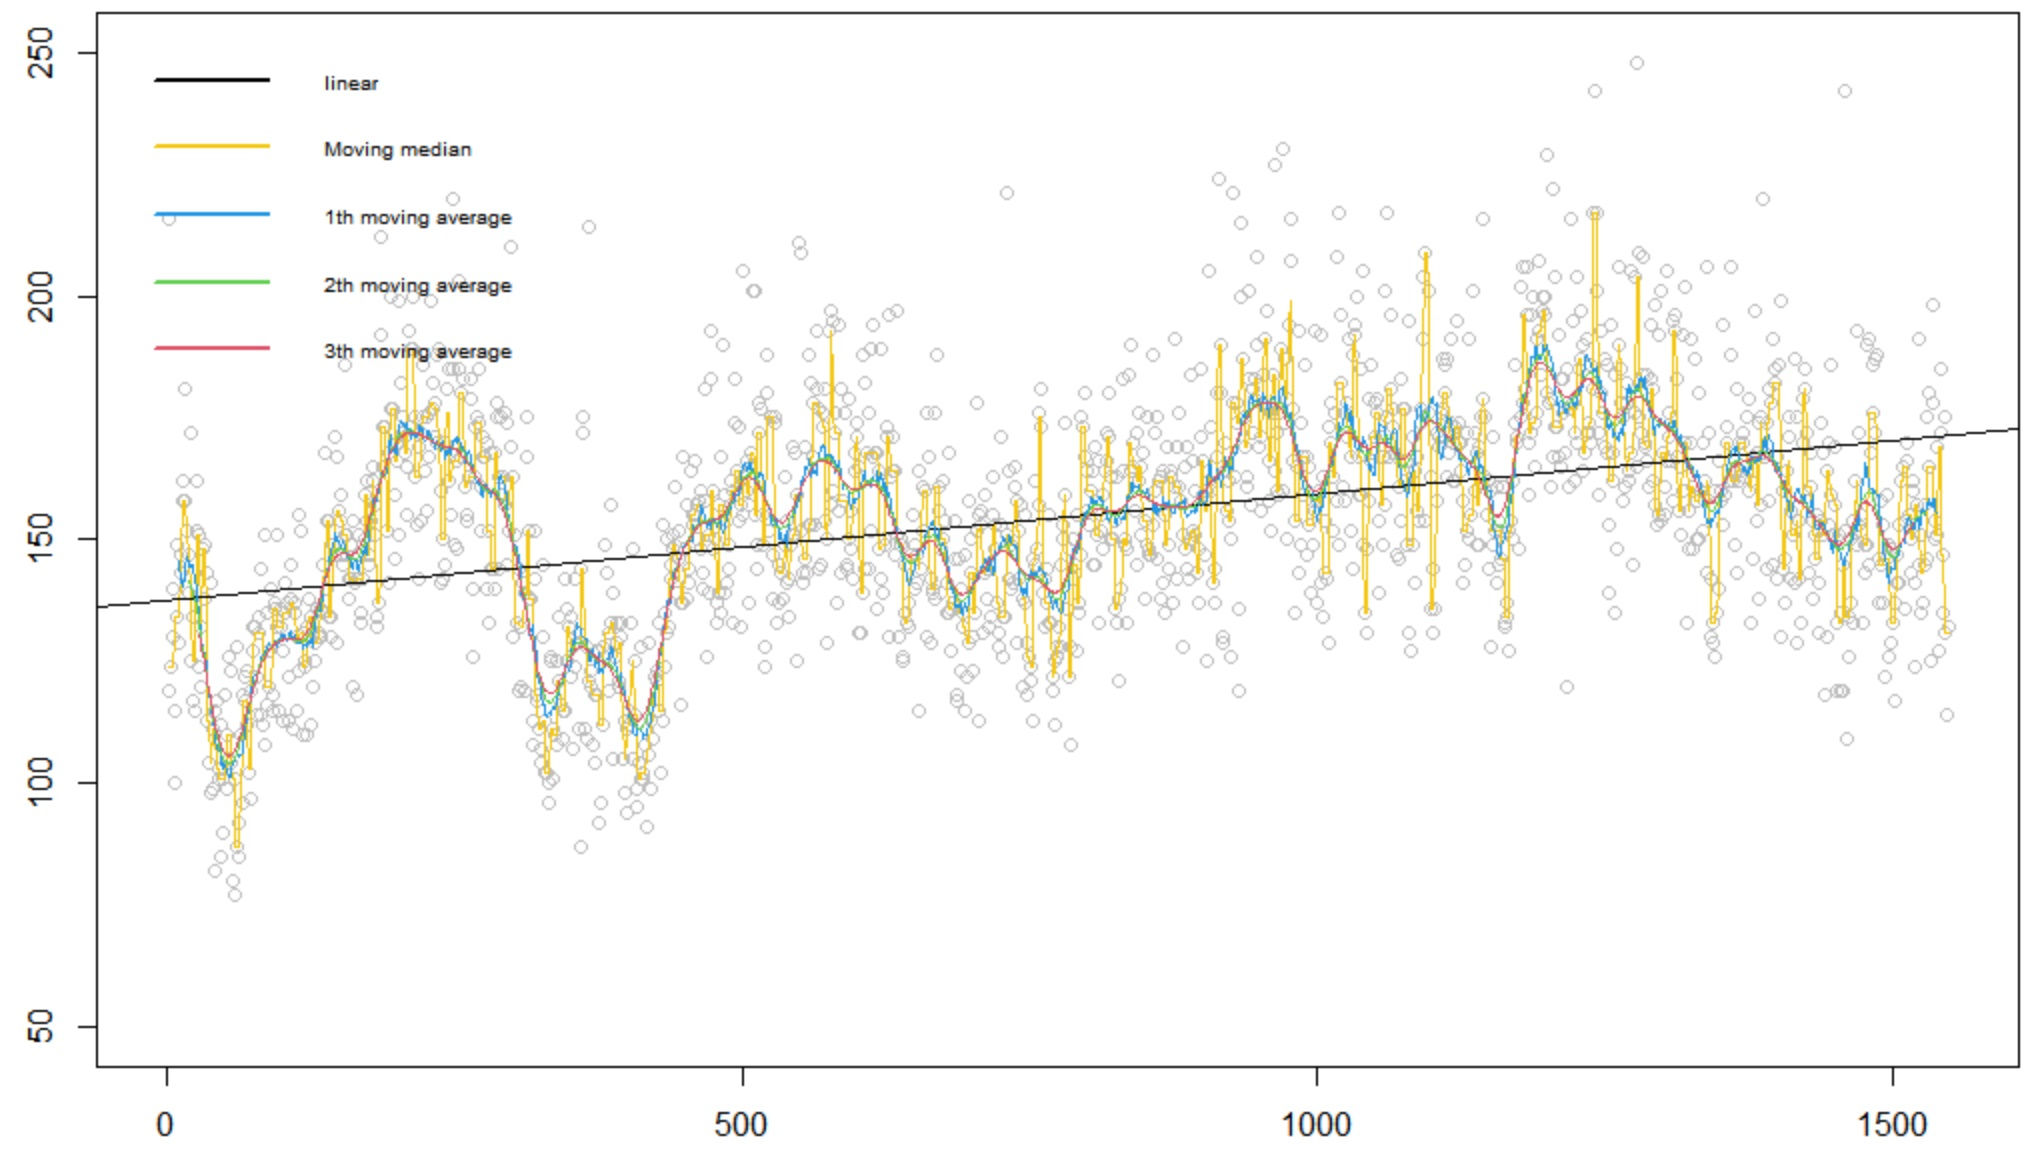
\includegraphics[width=0.7\textwidth]{hua.jpg} %1.png是图片文件的相对路径
	\caption{时间序列中光滑方法} %caption是图片的标题
\end{figure}

可以看到移动中值法的光滑效率是不如移动平均的,在选择滤波器宽度为20的情况下,三次滑动平均后就可以得到很光滑的曲线了\cite{Tukey}。

常用的光滑方法还有多项式拟合,但是这里由于波动太频繁太大,所以不是很适合。可以考虑核回归的方式,对于每个点由核函数给每个样本点权重后进行计算回归后的值,可以看到光滑效果很好。同时考虑应用广泛的样条函数进行光滑,这里采用了自然样条和B-样条两种样条,都取相同的结点数量,并在一张图中(图五)展示。

\begin{figure}[!htb]
	\centering
	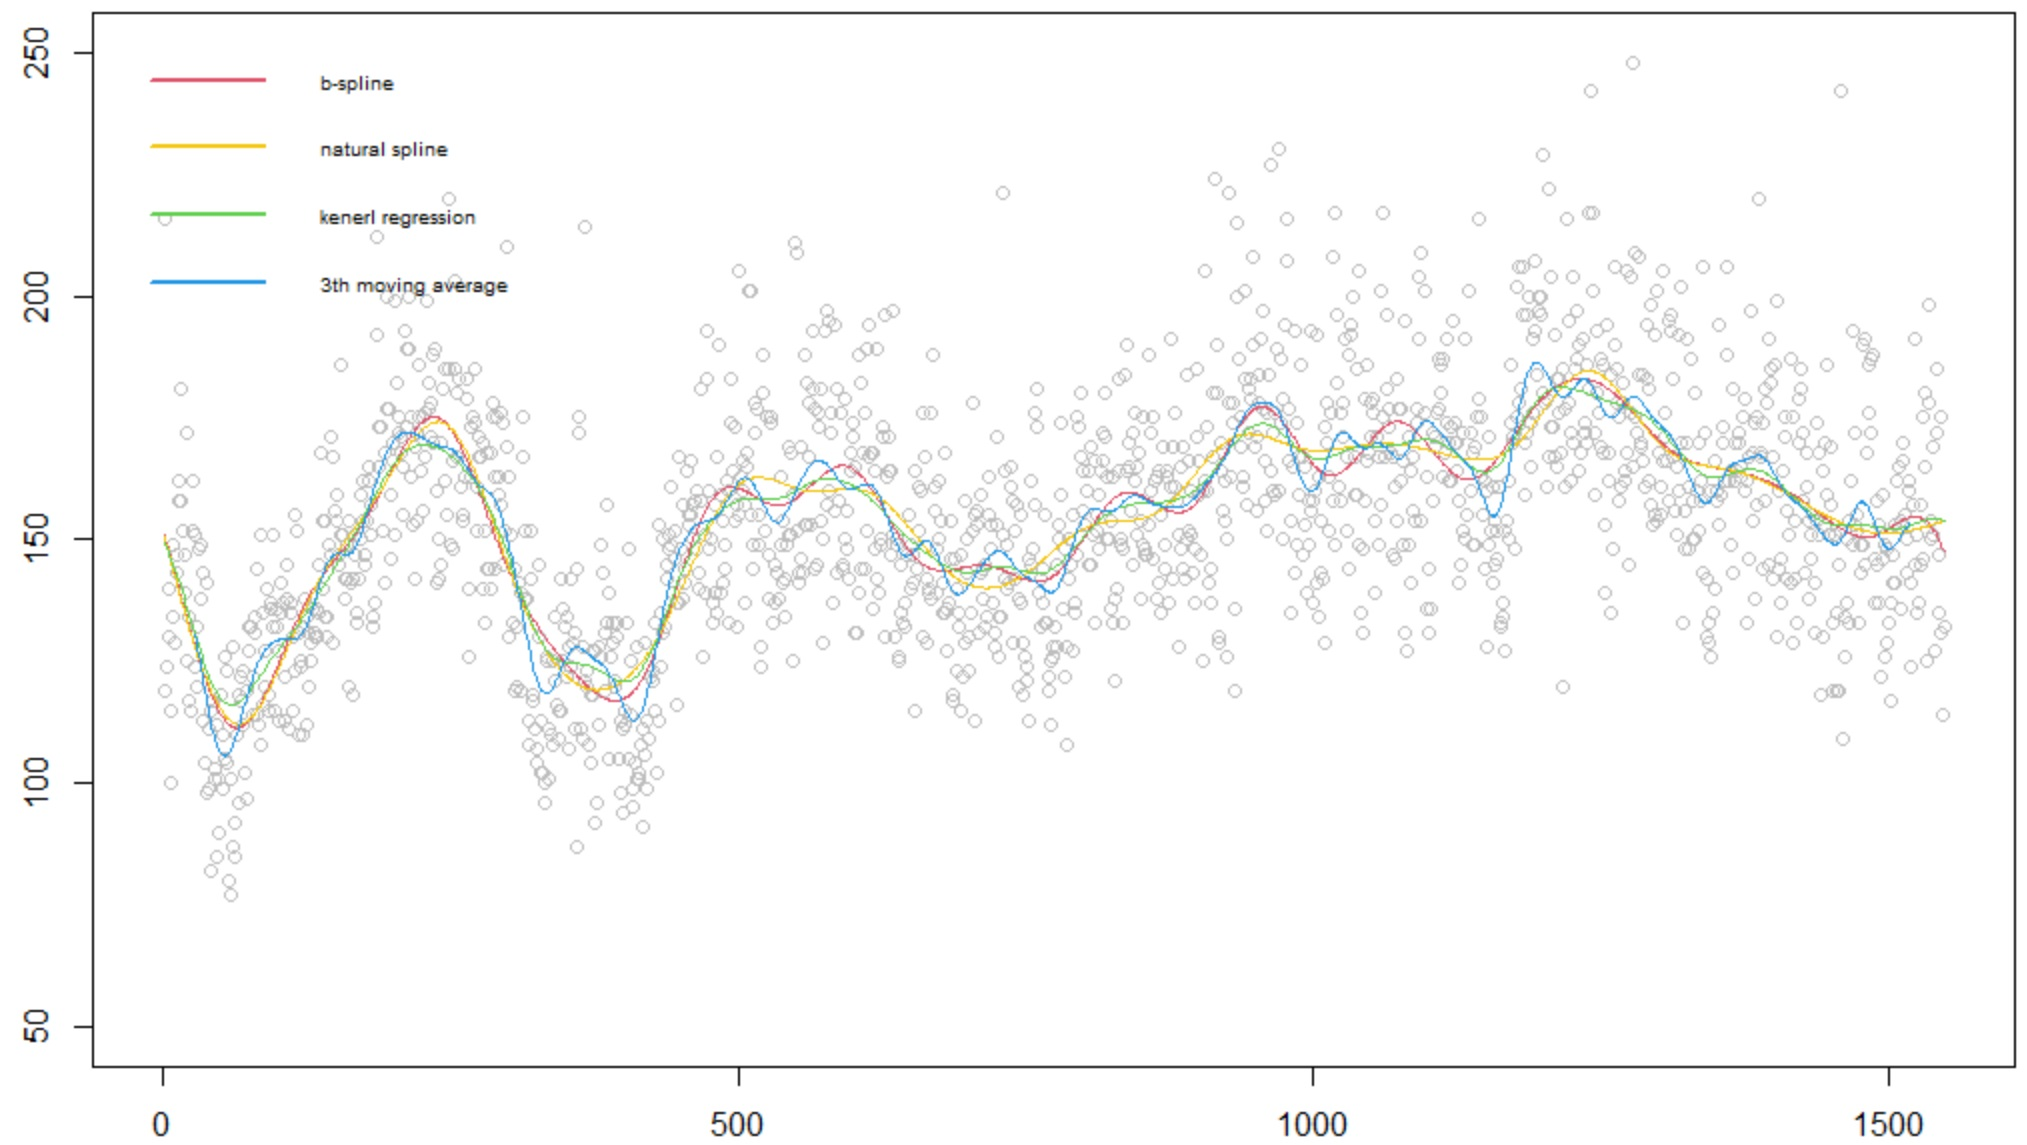
\includegraphics[width=0.7\textwidth]{spline.jpg} %1.png是图片文件的相对路径
	\caption{核回归方法和样条法} %caption是图片的标题
\end{figure}
可以看到自然样条在边界比B样条更加控制,这是因为自然样条在边界施加了限制。可以看到核回归和滑动平均比更加地平滑,考虑这是因为核回归考虑到了更多样本点,而滑动平均考虑到邻近的点。但是这些光滑方法在此问题中都比较好地解决了光滑问题。为进一步分析提供了支持。
\begin{figure}[!htb]
	\centering
	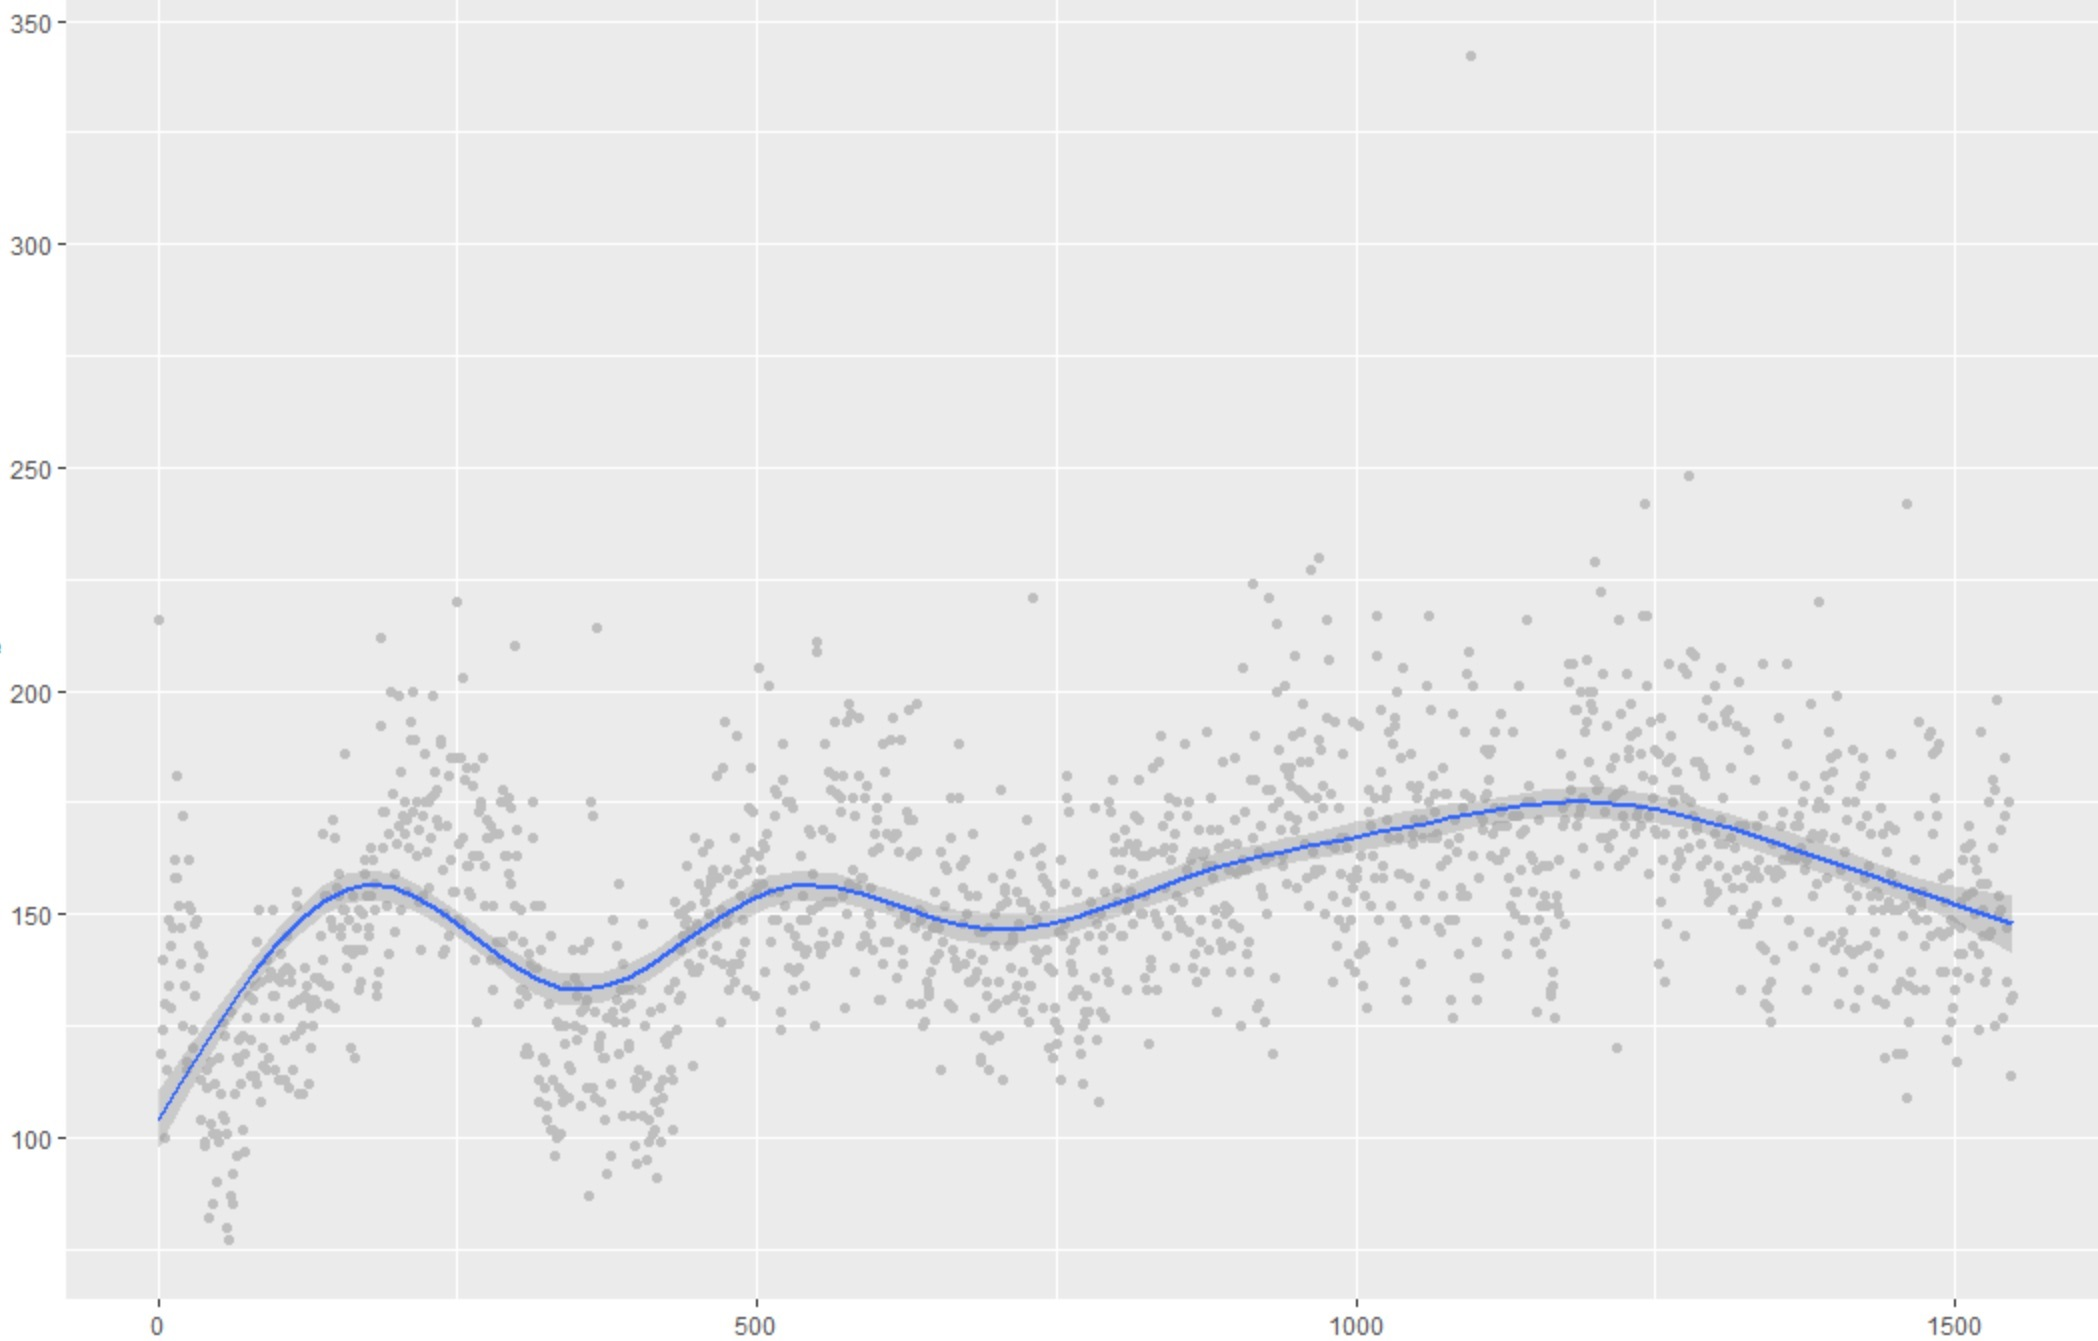
\includegraphics[width=0.5\textwidth]{gam.jpg} %1.png是图片文件的相对路径
	\caption{GAM} %caption是图片的标题
\end{figure}
这里进一步考虑广义加性模型(GAM)模型\cite{Bo},广义相加模型通过光滑样条函数 、核函数或者局部回归光滑函数,对变量进行拟合。GAM采用模型中的每个预测变量并将其分成多个部分(由'结'​​分隔),然后将多项式函数分别拟合到每个部分。GAM的原理是最小化残差(拟合优度)同时最大化简约性(最低可能自由度)。见图六,可以看到更好的光滑程度,但是可能丧失更多信息。


\subsection{枪击案件的空间规律}
\begin{figure}[!htb]
	\centering
	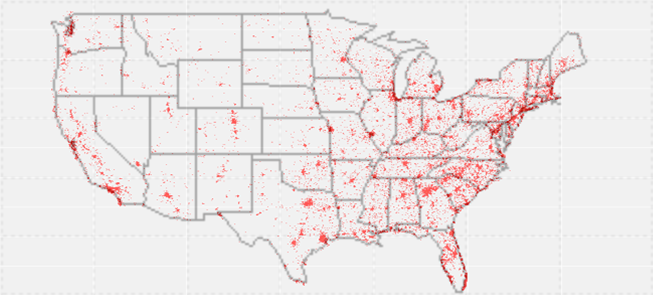
\includegraphics[width=0.7\textwidth]{dot.png} %1.png是图片文件的相对路径
	\caption{枪击案分布图} %caption是图片的标题
	
	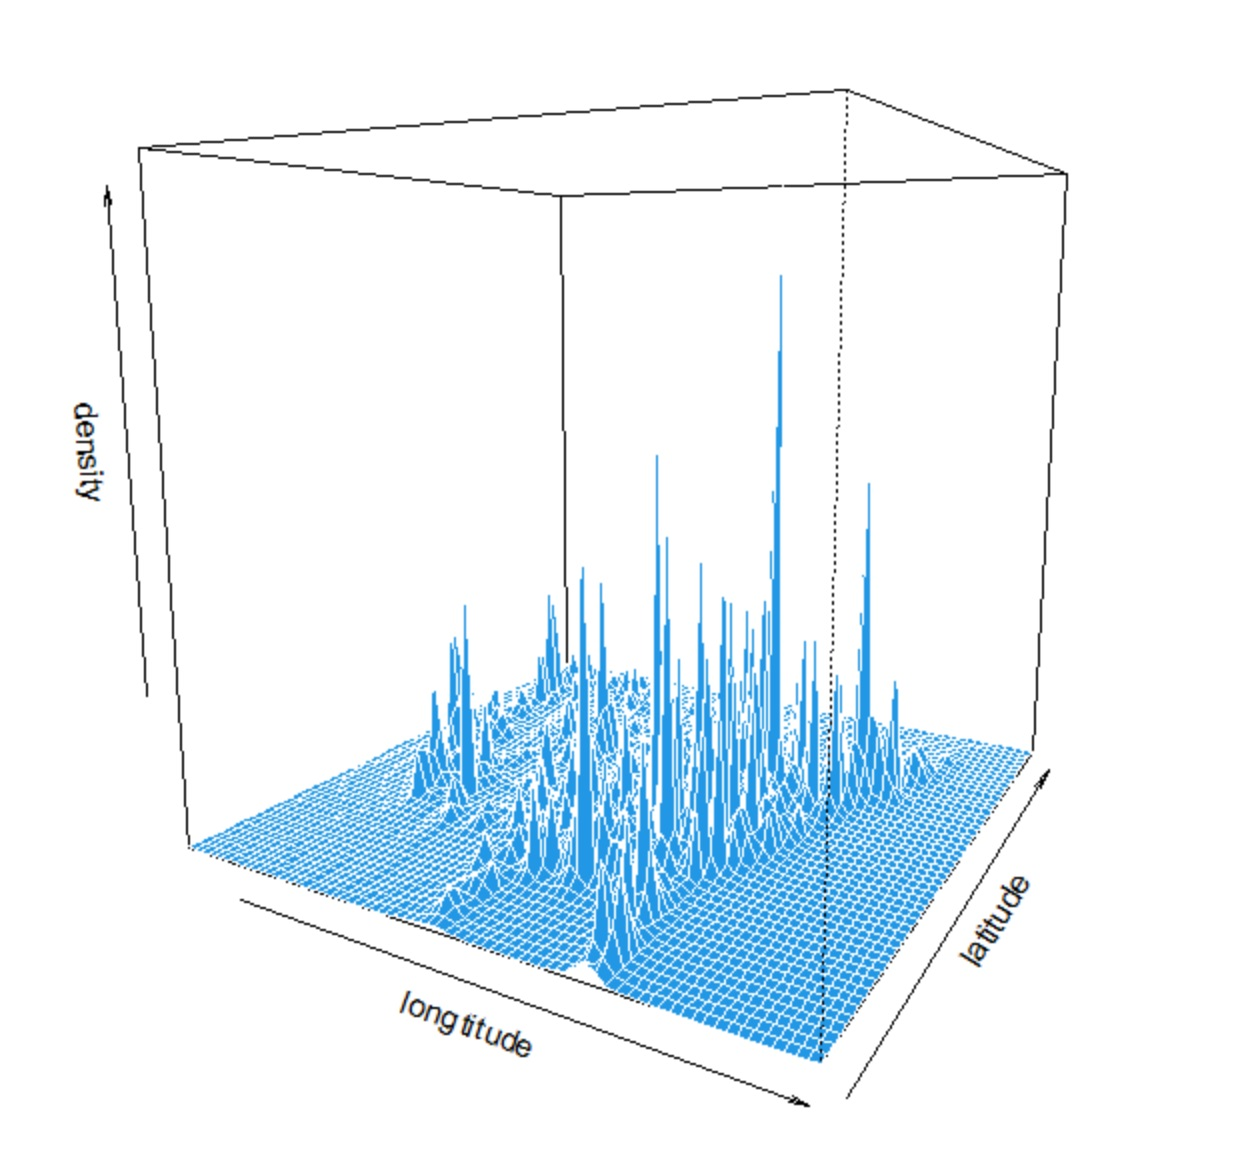
\includegraphics[width=0.7\textwidth]{per.jpg} %1.png是图片文件的相对路径
	\caption{最近邻估计} %caption是图片的标题
\end{figure}
美国人普遍持枪,那么枪击案发生是不是单纯只是和人口分布密度有关,和那些地区地枪击案可能性比较高,这可以为政府政策制定提供了导向。很自然的想法就是在在地图上对案件发生地进行标注,形成时间发生分布图,事件越密集的地区那么意味着枪击案发生的概率更高。在gun-violence数据集中提供绝大部分案件的经纬度,所以可以由经纬度画出散点图,并与美国地图进行合成,得到了分布图(图七)。

但是这种分布图因为只能靠感觉去估计案件发生的可能性,所以更希望能通过更直观的一种方式去进行估计发生的概率。这里先通过二维最近邻密度估计进行密度估计,这种方式是通过欧式距离最近的前几个点进行估计。



通过可视化(图八),可以发现在西经83度北纬40度附近的枪击案件发生的是最频繁的。 即伊利诺伊州和印第安纳州交界处。
并且枪击案发生分布很不均匀,在某些地区呈现一种很高枪击发生率的状态。 接下来可以通过很常用的核密度估计,并且将密度图和美国地图进行合成,得到更加直观的结果。这种处理方法在犯罪率数据的处理上很常见。

\begin{figure}[!htb]
	\centering
	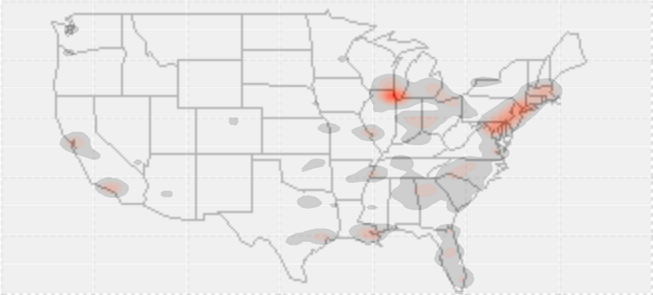
\includegraphics[width=0.7\textwidth]{den.png} %1.png是图片文件的相对路径
	\caption{密度图} %caption是图片的标题
\end{figure}



\subsection{数据分析结果}


\section{结论}
根据所作分析,可以得到案件频率发生总体来说是高度符合正态分布的,这也和现实中枪击案件是大量的复杂地相互影响造成地相吻合。从时间角度来看,整体枪击案件的频率是上升趋势的,并且每年年中是枪击案件的高发时间。这和Matthew Ranson的气温高越容易犯罪的理论是契合的\cite{Ranson M}。从空间上来看,可以发现枪击案发生地分布不均匀,集中分布在密西根湖和东海岸附近。但是这和美国人口分布并不是重叠的,但和犯罪率分布却高度重叠。这说明枪支和犯罪高度关联,控制枪支对于美国控制犯罪有很大的意义。





%\renewcommand{\baselinestretch}{1.1}
\normalsize
\begin{thebibliography}{}


\bibitem[1]{Tukey}
Tukey J W . Exploratory Data Analysis[J]. Journal of the American Statistical Association, 1977, 28(1).

\bibitem[2]{Bo}
Bo, E, H, et al. Generalized standard addition method[J]. Analytical Chemistry, 1979.

\bibitem[3]{Ranson M}
Ranson M . Crime, weather, and climate change[J]. Journal of Environmental Economics and Management, 2014, 67(3):274-302.


\end{thebibliography}


\section*{附录}
所有数据和代码均已上传https://github.com/mayiming24/gun.git


\end{document}
